% \documentclass[final,5p,times,twocolumn]{elsarticle}
% \def\tablename{Table}%
% %\usepackage{flushend}
% \usepackage{amssymb}
% \usepackage{amsmath}
% \usepackage{subfigure}
% \journal{DCA}
% \begin{document}
%
% \begin{frontmatter}
% \title{Visual Adaptive Control of Planar Robots Manipulators of two linkages using Neuro-control based in spikes.}
%
% \author[First]{Perrusqu\'ia Guzm\'an, J. \corref{cor1}}
% \ead{jperrusquia@ctrl.cinvestav.mx}
%
% \author[Second]{Reyes S\'amano, A.}
% \ead{areyes@ctrl.cinvestav.mx}
%
% \cortext[cor1]{Author's data}
%
% \address[First]{Departamento de Control Autom\'atico, CINVESTAV-IPN, Av. IPN 2508,07360 M\'exico, M\'exico.}
% \address[Second]{Departamento de Control Autom\'atico, CINVESTAV-IPN, Av. IPN 2508,07360 M\'exico, M\'exico.}
%
% \begin{abstract}
% In this work is proposed an adaptive control of planar robots using neurocontrol based in spikes. The adaptive control is well known and its functionality has been demonstrated. We present the design of a brain that makes the functionality of the adaptive control using a neural simulator called ``Nengo'' and brain's communication theory.
% \end{abstract}
%
% \begin{keyword}
% Robot Manipulator \sep Adaptive Control \sep Regressor \sep  Adaptive law \sep Ensembles \sep Linear Transform \sep Non linear Transform \sep Integrator.
%
%
% \end{keyword}
%
% \end{frontmatter}

\section{Introduction}
Brains are fantastic devices. For one, they are incredibly efficient. Brains consume only about 20 watts(W) of power- the equivalent of a compact fluorescent light bulb.\\

In general, it is believed that what provides brains with their impressive computational abilities is the organization of the connections among individual neurons. These connections allow cells to collect, process, and transmit information. In fact, neurons are specialized precisely for communication. In most respects, neurons are exactly like other cells in our bodies- they have a cell membrane, a nucleus, and similar metabolic process. \\

\begin{figure}[h]
\centering
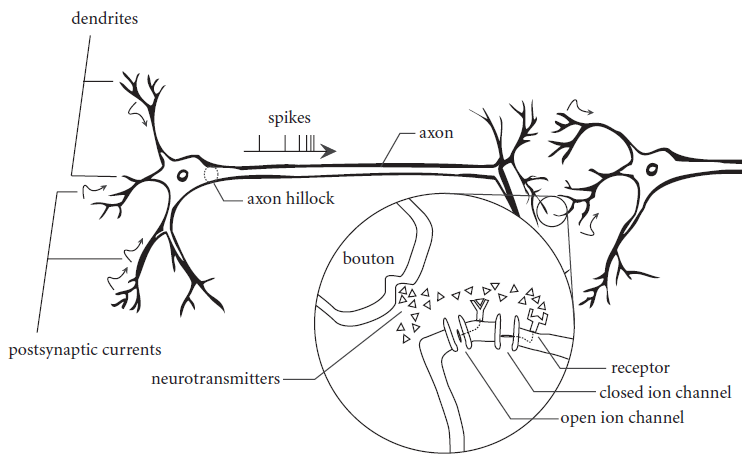
\includegraphics[width=0.45\textwidth]{imagenes/6-neuronal/transmision.png}
 \caption{The main elements of neural communication}
 \label{fig:cerebro}
\end{figure}
Figure \ref{fig:cerebro} outlines the main elements underlying cellular communication. The cellular projections that carry information to the cell body are called dendrites. The cellular projection that carries information away from the cell body in called the axon. Dendrites carry signals to the cell body in the form of an ionic current. If sufficient current gathers in the cell body (at the axon hillock), then a series of cellular events are triggered that result in an action potential, or voltage ``spike'', that proceeds down the axon. Neural spikes are very brief events lasting for only about a millisecond, which travel in a wave-like fashion down the axon until they reach the end of the axon, called the bouton. When spikes reach the bouton, they cause the release of tony packets of chemicals called neurotransmitters into the space between the bouton and the dendrite of the subsequent neuron. The neurotransmitters the bind to special proteins called ``receptors'' in the cell membrane of the dendrite. This binding causes small gates, or channels, in the dendrite of the next neuron to open, allowing charged ions to flows into the dendrite. These ions result in the current signal in the receiving dendrite, which is called the postsynaptic current (PSC, see Figure \ref{fig:spike}). The process then continues as it began.\\

\begin{figure}[h]
\centering
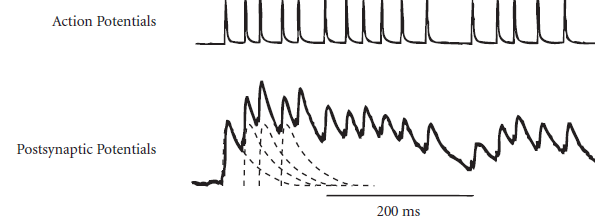
\includegraphics[width=0.45\textwidth]{imagenes/6-neuronal/spike.png}
 \caption{Electrical activity in two connected neurons}
 \label{fig:spike}
\end{figure}

Using this theory we pretend to develop an adaptive control of a planar robot. The result is a control scheme using a brain model.
\section{The Robot Manipulator}
The dynamic model of a rigid serial $n$-link nonredundant manipulator with all actuated revolute joints describes in generalized joint coordinates $(q^T,\dot{q}^T)^T\in\mathbb{R}^{2n}$ can be written as follows,

\begin{equation}
M(q)\ddot{q}+C(q,\dot{q})\dot{q}+G(q)=\tau\label{din}
\end{equation}

where $M(q)\in\mathbb{R}^{n\times n}$ denotes a symmetric positive definite inertial matrix, $C(q,\dot{q})\in\mathbb{R}^{n\times n}$ stands for the Coriolis and centrifugal forces matrix, $G(q)\in\mathbb{R}^n$ models the gravity forces, $\tau\in\mathbb{R}^n$ stands for the torque input.

\section{Adaptive Control}
The nonlinear robot dynamics is linearly parametrizable \citep{Slotine} by the product of a regressor $Y=Y(q,\dot{q},\ddot{q})\in\mathbb{R}^{n\times p}$ which is a function of joint positions, velocities and accelerations, and a vector $\Theta\in\mathbb{R}^{p\times1}$ of constant parameters, as follows:

\begin{equation}
M(q)\ddot{q}+C(q,\dot{q})\dot{q}+G(q)=Y(q,\dot{q},\ddot{q})\Theta=\tau\label{din2}
\end{equation}

Consider the control law \citep{Adapt}

\begin{equation}
\tau=M(q)\ddot{q_r}+C(q,\dot{q})\dot{q_r}+G(q)+K_D\sigma\label{mal}
\end{equation}

with $K_D$ a positive definite matrix. The choice

\begin{equation}
\dot{q_r}=\dot{q_d}+\Lambda \tilde{q} \ \ \ \ \ddot{q_r}=\ddot{q_d}+\Lambda \dot{\tilde{q}}
\end{equation}

with $\Lambda$ a positive definite (usually diagonal) matrix, allows expressing the nonlinear compensation and decoupling terms as a function of the desired velocity and acceleration, corrected by the current state ($q$ and $\dot{q}$) of the manipulator. In fact, notice that the term $\dot{q_r}=\dot{q_d}+\Lambda \tilde{q}$ weighs the contribution that depends on velocity not only on the basis of the desired velocity but also on the basis of the position tracking error.\\

The term $K_D\sigma$ is equivalent to a PD action on the error if $\sigma$ is taken as

\begin{equation}
\sigma=\dot{q_r}-\dot{q}=\dot{\tilde{q}}+\Lambda\tilde{q}
\end{equation}

The control law (\ref{mal}) assumes that the parameters of the manipulator are known. The control law can be made \textit{adaptive} with respect to the vector of parameters $\Theta$, i.e., the parameters are not known exactly. The control law (\ref{mal}) is then modified into

\begin{align}
\tau&=\hat{M}(q)\ddot{q_r}+\hat{C}(q,\dot{q})\dot{q_r}+\hat{G}(q)+K_D\sigma\nonumber\\
&=Y(q,\dot{q},\dot{q_r},\ddot{q_r})\hat{\Theta}+K_D\sigma\label{control}
\end{align}

where $\hat{\Theta}$ represents the available estimate on the parameters and, accordingly $\hat{M},\hat{C},\hat{G}$ denote the estimate terms in the dynamic model. Substituting control (\ref{control}) into (\ref{din}) gives

\begin{align}
M(q)\dot{\sigma}+C(q,\dot{q})\sigma+K_D\sigma&=-\tilde{M}(q)\ddot{q_r}-\tilde{C}(q,\dot{q})\dot{q_r}-\tilde{G}(q)\nonumber\\
&=-Y(q,\dot{q},\dot{q_r},\ddot{q_r})\tilde{\Theta},\label{tray}
\end{align}

the modeling error is characterized by:

\begin{equation}
\tilde{M}=\hat{M}-M, \ \ \ \ \ \tilde{C}=\hat{C}-C, \ \ \ \ \ \tilde{G}=\hat{G}-G, \ \ \ \ \ \tilde{\Theta}=\hat{\Theta}-\Theta
\end{equation}

Notice that the matrix $Y$ does not depend on the actual joint accelerations but only on their desired values; this avoids problems due to direct measurement of acceleration.\\

Consider the Lyapunov function candidate

\begin{equation}
V(\sigma,\tilde{q},\tilde{\Theta})=\frac{1}{2}\sigma^T M(q)\sigma+\tilde{q}^T\Lambda K_d \tilde{q}+\frac{1}{2}\tilde{\Theta}^T K_{\Theta} \tilde{\Theta}>0 \label{lyap}
\end{equation}

where the first term is the kinetic energy, the introduction of the second and third term in (\ref{lyap}) are necessary to obtain a Lyapunov function of the entire system state. The second term vanishes for $\tilde{q}=0$, and the third term is for the parameter error, with $K_\Theta$ symmetric positive definite. The time derivative of $V$ along the trajectories of system (\ref{tray}) is

\begin{equation}
\dot{V}=-\dot{\tilde{q}}^T K_D \dot{\tilde{q}}-\tilde{q}^T \Lambda K_D \Lambda\tilde{q}+\tilde{\Theta}^T\left(K_{\Theta}\dot{\tilde{\Theta}}-Y^T(q,\dot{q},\dot{q_r},\ddot{q_r})\sigma\right)\label{lyap2}
\end{equation}

If the estimate of the parameter vector is updated as in the adaptive law

\begin{equation}
\dot{\hat{\Theta}}=K_{\Theta}^{-1}Y^T(q,\dot{q},\dot{q_r},\ddot{q_r})\sigma\label{adap}
\end{equation}

the expression in (\ref{lyap2}) becomes

\begin{equation}
\dot{V}=-\dot{\tilde{q}}^T K_D \dot{\tilde{q}}-\tilde{q}^T \Lambda K_D \Lambda \tilde{q}
\end{equation}

since $\dot{\hat{\Theta}}=\dot{\tilde{\Theta}}$ ($\Theta$ is constant).\\

The trajectories of the manipulator described by the model (\ref{din}), under the control law (\ref{control}) and the parameter adaptive law (\ref{adap}), globally asymptotically converge to $\sigma=0$ and $\tilde{q}=0$, which implies convergence to zero of $\tilde{q},\dot{\tilde{q}}$, and boundedness of $\hat{\Theta}$. The equation in (\ref{tray}) shows that asymptotically it is

\begin{equation}
Y(q,\dot{q},\dot{q_r},\ddot{q_r})\left(\hat{\Theta}-\Theta\right)=0
\end{equation}

This equation doesn't imply that $\hat{\Theta}$ tends to $\Theta$; indeed, convergence parameters to their true values depends on the structure of the matrix $Y(q,\dot{q},\dot{q_r},\ddot{q_r})$ and then on the desired and actual trajectories. To summarize:

\begin{itemize}
\item[$\bullet$] The term $Y\hat{\Theta}$ describes a control action of inverse dynamics type which ensures an approximate compensation of nonlinear effects and joint decoupling.
\item[$\bullet$] The term $K_D\sigma$ introduces a stabilizing linear control action of PD type on the tracking error.
\item[$\bullet$] The vector of parameter estimates $\hat{\Theta}$ is updated by an adaptive law of gradient type so as to ensure asymptotic compensation of the terms in the manipulator dynamic model; the matrix $K_\Theta$ determines the convergence rate of parameters to their asymptotic values.
\end{itemize}

\section{The Nengo Neural Simulator}
Nengo\citep{brain} is a graphical ans scripting bases software package for simulating large-scale neural systems. To use Nengo, you define groups of neurons in terms of what they represent, and then form connections between neural groups in terms of what computation should be performed on those representations. Nengo then uses the Neural Engineering Framework (NEF) to solve for the appropriate synaptic connection weights to achieve this desired computation.\\

The following three principles form the core of the NEF:

\begin{enumerate}
\item Neural representations are defined by the combination of nonlinear
encoding (exemplified by neuron tuning curves and neural spiking) and
weighted linear decoding (over populations of neurons and over time).
\item Transformations of neural representations are functions of the variables
represented by neural populations. Transformations are determined
using an alternately weighted linear decoding.
\item Neural dynamics are characterized by considering neural
representations as state variables of dynamic systems. Thus, the
dynamics of neurobiological systems can be analyzed using control (or
dynamics systems) theory.
\end{enumerate}

To program the controller using Nengo we used the scripting system. The scripting system used in Nengo is Python. Firstly we need to consider the next information:

\begin{itemize}
\item The control task is for regulation, then
$$\dot{q_d}=0 \ \ \ \ \mbox{and} \ \ \ \ \ddot{q_d}=0$$
\item The robot manipulator has reduction gear, then the velocity is small and the Coriolis elements are despicable.
\end{itemize}

With this consideration the regressor is easier to compute in Nengo. The elements we need to use for the controller compute are:

\begin{enumerate}
\item \textbf{Function}: this created an input function. In our case will be constant functions that represents values of the actual and desired joints.
\item \textbf{Ensemble}: this is generated my the user according to the operation we want to make, with a certain number of neurons, radio and dimension. This element is the most used for the controller design.
\item \textbf{Integrator}: its similar to the ensemble, the difference is that this ensemble makes the integral of the ensemble. It was use for the adaptive law.
\item \textbf{Array of ensembles}: When building models that represent large numbers of dimensions, it is sometimes useful to break an ensemble down
into sub-ensembles, each of which represent a subset of dimensions. The main advantage of this is speed: It is much faster for the NEF methods to compute decoders for many small
ensembles, rather than one big one.
\end{enumerate}

From all the tools that provides Nengo, we only used linear transformations and non linear transformations. In Figure \ref{fig:error} shows the joint position error using Nengo.\\

\begin{figure}[h]
\centering
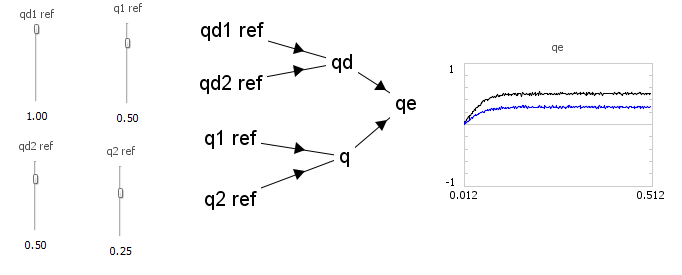
\includegraphics[width=0.45\textwidth]{imagenes/6-neuronal/error.png}
 \caption{Joint position error using Nengo}
 \label{fig:error}
\end{figure}

\section{Digital Simulations}
In this section, the robot manipulator ans its dynamic parameters, the simulation setup, and results are presented and discussed.

\begin{figure}[h]
\centering
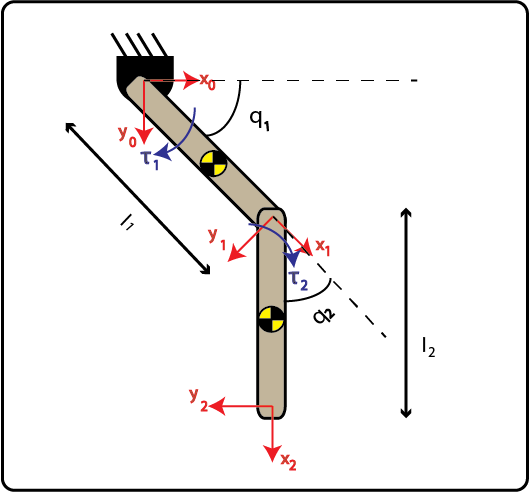
\includegraphics[width=0.35\textwidth]{imagenes/6-neuronal/pendubot.png}
 \caption{Joint position error using Nengo}
 \label{fig:error}
\end{figure}

The regressor is given by:

\begin{equation}
Y=\left[\begin{array}{cccc}
y_{11}&y_{12}&y_{13}&y_{14}\\
y_{21}&y_{22}&y_{23}&y_{24}
\end{array}\right]
\end{equation}

and their values are:

\begin{align*}
y_{11}=&l_1^2\ddot{q_{r_1}}+\frac{1}{2}gl_1\cos(q_1)\\
y_{12}=&\left(l_1^2+l_2^2+2l_1l_2\cos(q_2)\right)\ddot{q_{r_1}}+\left(l_2^2+l_1l_2\cos(q_2)\right)\ddot{q_{r_2}}\\
&+\frac{1}{2}gl_2\cos(q_1+q_2)\\
y_{13}=&\ddot{q_{r_1}}\\
y_{14}=&\ddot{q_{r_1}}+\ddot{q_{r_2}}\\
y_{21}=&0\\
y_{22}=&\left(l_2^2+l_1l_2\cos(q_2)\right)\ddot{q_{r_1}}+l_2^2\ddot{q_{r_2}}-\frac{1}{2}gl_2\cos(q_1+q_2)\\
y_{23}=&0\\
y_{24}=&\ddot{q_{r_1}}+\ddot{q_{r_2}}
\end{align*}

The kinematics parameters are given in the Table \ref{tab1}:\\

\begin{table}[h]
\centering
\caption{Experimental robot parameters}
\label{tab1}
\begin{tabular}{|c|c|c|}
\hline
\bf{Symbol}&\bf{Parameter}&\bf{Value}\\\hline
$l_1$&Link 1&0.31m\\\hline
$l_2$&Link 2&0.305m\\\hline
\end{tabular}
\end{table}

Notice that we don't give the dynamical parameters such as mass and inertia. The estimate parameter vector $\hat{\Theta}$ contains the estimate value of mass and inertia for each link. In other words, the estimate parameter value is $\hat{\Theta}=\left[\begin{array}{cccc}m_1&m_2&I_1&I_2\end{array}\right]^T$, where $m_1$, $I_1$ are the mass and inertia from the link 1, and $m_2$, $I_2$ are the mass and inertia from the link 2. The parameters of control are given in the Table \ref{tab2}.

\begin{table}[h]
\centering
\caption{Parameters of control}
\label{tab2}
\begin{tabular}{|c|c|c|}
\hline
\bf{Gain}&\bf{Value}\\\hline
$\Lambda$&5\\\hline
$K_D$&5\\\hline
$K_\Theta$&20\\\hline
\end{tabular}
\end{table}

We considered $m_1=2$kg, $m_2=3{.}5$kg, $J_1=J_2=0$kg$\mbox{m}^2$. The simulations time was 20 seconds with an integration step of 1ms. The desired value is $\frac{\pi}{8}$.\\

\begin{figure}[h]
\centering
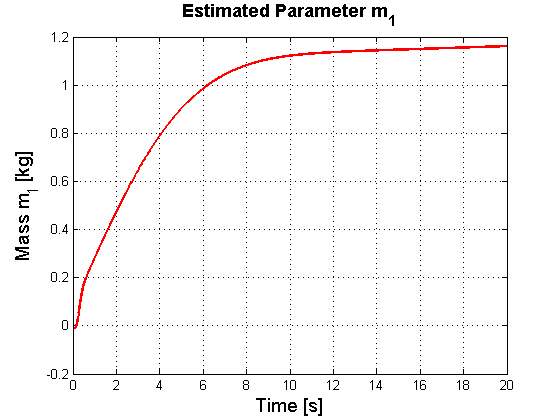
\includegraphics[width=0.38\textwidth]{imagenes/6-neuronal/m1.png}
 \caption{Estimated parameter $m_1$}
 \label{fig:m1}
 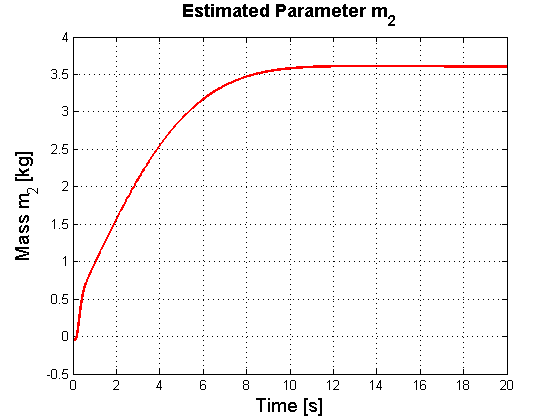
\includegraphics[width=0.38\textwidth]{imagenes/6-neuronal/m2.png}
 \caption{Estimated parameter $m_2$}
 \label{fig:m2}
\end{figure}

\begin{figure}[h]
\centering
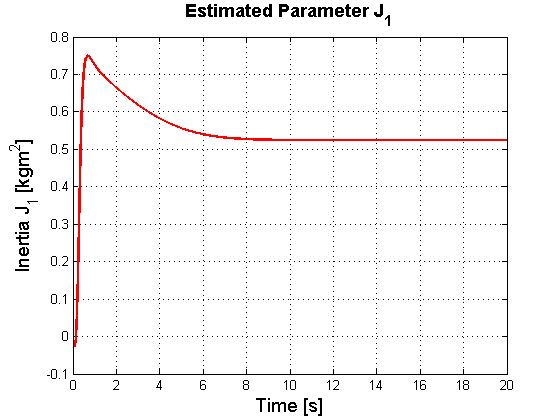
\includegraphics[width=0.38\textwidth]{imagenes/6-neuronal/J1.png}
 \caption{Estimated parameter $J_1$}
 \label{fig:J1}
 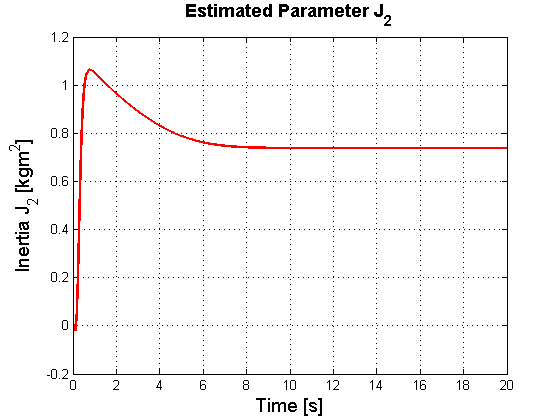
\includegraphics[width=0.38\textwidth]{imagenes/6-neuronal/J2.png}
 \caption{Estimated parameter $J_2$}
 \label{fig:J2}
\end{figure}

The previous Figures shows the estimate value of the mass and the inertia of each link. In a certain time the estimate parameter converges to their asymptotic values. In this simulation the asymptotic values are: $m_1\approx1{.}5$ kg, $m_2\approx3{.}5$ kg, $J_1\approx0{.}1$ kg$\mbox{m}^2$, and $J_2\approx0{.}18$kg$\mbox{m}^2$. This shows that $\hat{\Theta}$ doesn't tends to $\Theta$ but with the regressor ensure an approximate compensation of nonlinear effects ans joint decoupling.\\

\begin{figure}[h]
\centering
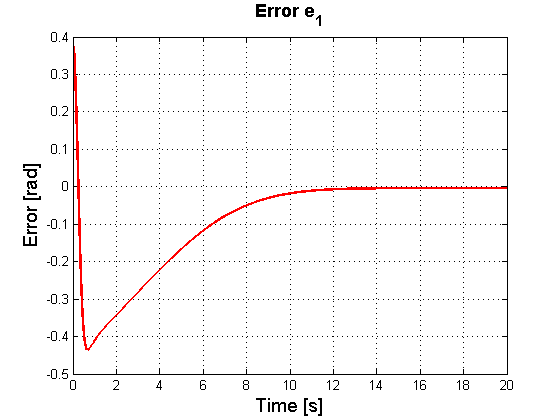
\includegraphics[width=0.38\textwidth]{imagenes/6-neuronal/e1.png}
 \caption{Joint error $e_1$ Adaptive Control}
 \label{fig:e1}
\end{figure}

\begin{figure}[h]
\centering
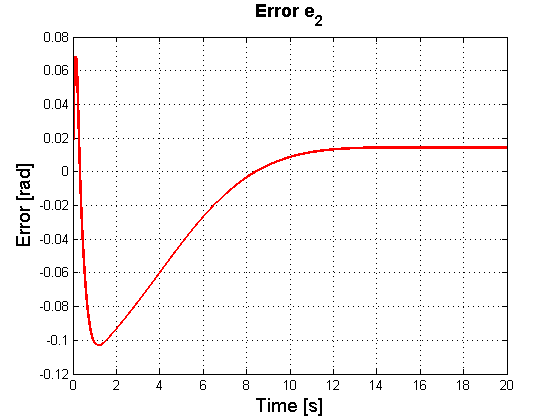
\includegraphics[width=0.38\textwidth]{imagenes/6-neuronal/e2.png}
 \caption{Joint error $e_2$ Adaptive Control}
 \label{fig:e2}
\end{figure}

\begin{figure}[h]
\centering
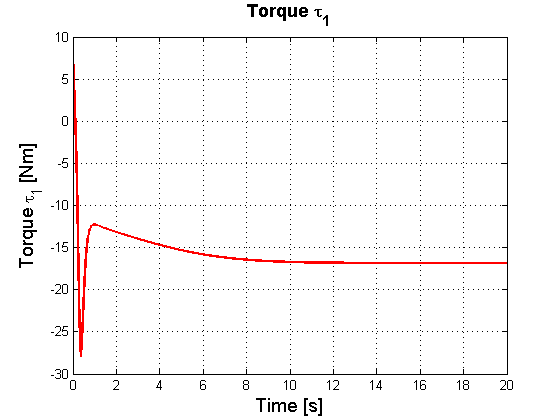
\includegraphics[width=0.38\textwidth]{imagenes/6-neuronal/T1.png}
 \caption{Torque input $\tau_1$ Adaptive Control}
 \label{fig:T1}
\end{figure}

\begin{figure}[h]
\centering
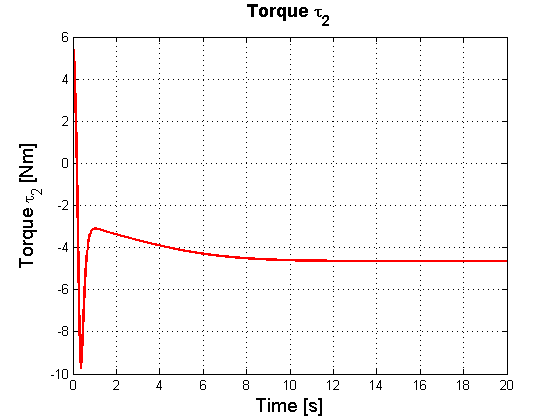
\includegraphics[width=0.38\textwidth]{imagenes/6-neuronal/T2.png}
 \caption{Torque input $\tau_2$ Adaptive Control}
 \label{fig:T2}
\end{figure}

The joint error (see Figure \ref{fig:e1} and \ref{fig:e2}) converges approximately to zero even the controller doesn't know the mass and inertia parameters. The torque inputs (see Figure \ref{fig:T1} and \ref{fig:T2}) have a  peak at the beginning cause the initial conditions, then the torque stabilize in a certain value.

\section{Nengo connecting problems}
When we got the program of the controller using Nengo, we wanted to exported to Matlab, but we got problems because Matlab didn't recognize the NEF, so we couldn't see if our brain can make the adaptive control. We started to compare the values  of the output of the regressor and the joint errors without connecting to the robot manipulator. The result was that are approximately the same, but when we compared the output of the integrator, it was unstable and their values tended to infinity.\\

To provide a comparison between the controller in Nengo and Matlab we make a PD+G controller,

\begin{equation}
\tau=K_Pe(t)+K_D\dot{e}(t)+G(q)
\end{equation}

with $K_P, K_D$ a positive definite matrix (proportional gain and derivative gain) and $G(q)$ is the vector of gravity forces. $e(t)$ in the joint position error, $e(t)=q_d-q$, and $\dot{e}(t)$ is the joint velocity error, $\dot{e}(t)=\\dot{q_d}-\dot{q}$. This controller is easier than the adaptive control and can give us the information we need to compare Matlab simulation and Nengo simulation.\\

For this controller we need to provide the values of the mass. The desired value was $\frac{\pi}{2}$ with the same time of simulation but the gain parameters are given by the Table \ref{tab3}.\\

\begin{table}[h]
\centering
\caption{Parameters of control PD+G}
\label{tab3}
\begin{tabular}{|c|c|c|}
\hline
\bf{Gain}&\bf{Value}\\\hline
$K_P$&3\\\hline
$K_D$&3\\\hline
\end{tabular}
\end{table}

In the simulation with Nengo show that the torque input are approximately the same as Matlab Simulation (see Figure \ref{fig:t}).\\

\begin{figure}[h]
\centering
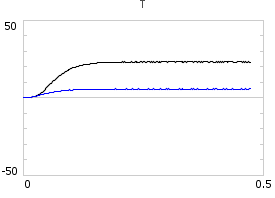
\includegraphics[width=0.3\textwidth]{imagenes/6-neuronal/t.png}
 \caption{Torque input $\tau$ PD+G in Nengo}
 \label{fig:t}
\end{figure}

The joint error (see Figure \ref{fig:e1g} and Figure \ref{fig:e2g}) converges to zero because in this case we known the parameters and the  gravity forces vector of the controller compensates the gravity terms of the manipulator.\\

The torque inputs have a maximum value by the same reason of the initial conditions, then the torque stabilize in cero. Notice that the PD+G action is more smoothly than the adaptive control. But the disadvantage of this control is that we need to know the parameters of the manipulator.\\

\begin{figure*}[tb]
\centering
\subfigure[Joint error $e_1$]{
   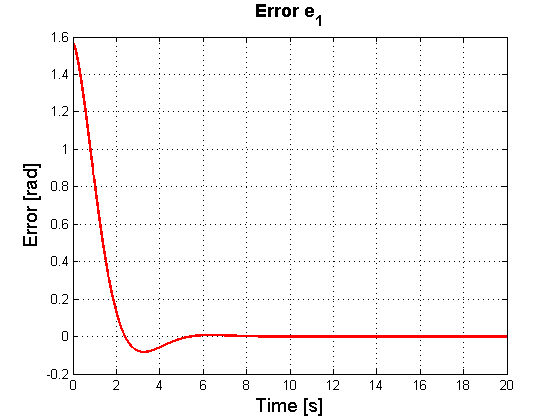
\includegraphics[scale =0.45] {imagenes/6-neuronal/e1g.png}
   \label{fig:e1g}
 }
 \subfigure[Joint error $e_2$]{
   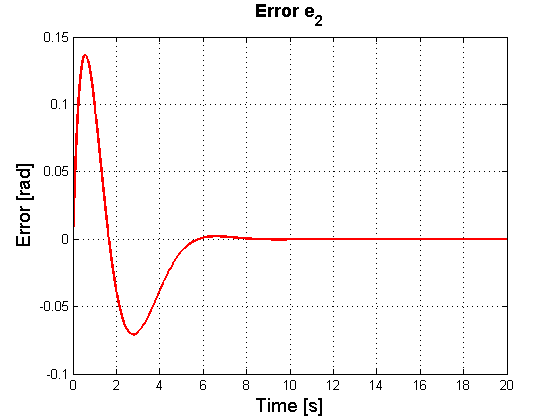
\includegraphics[scale =0.45] {imagenes/6-neuronal/e2g.png}
   \label{fig:e2g}
 }
 \subfigure[Torque input $\tau_1$]{
   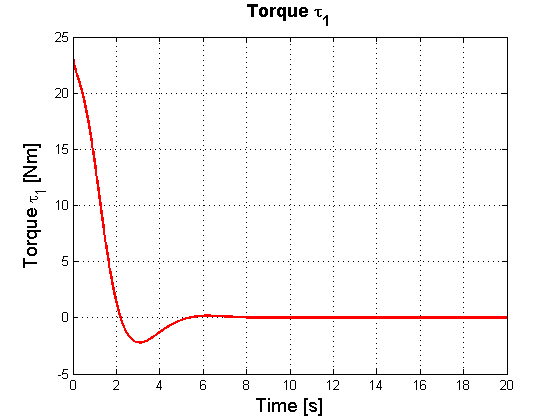
\includegraphics[scale =0.45] {imagenes/6-neuronal/T1g.png}
   \label{fig:T1g}
 }
 \subfigure[Torque input $\tau_2$]{
   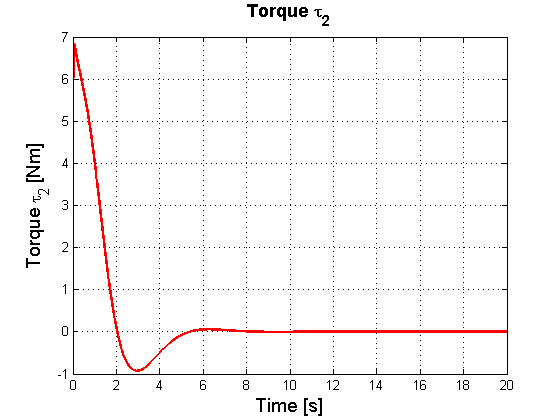
\includegraphics[scale =0.45] {imagenes/6-neuronal/T2g.png}
   \label{fig:T2g}
 }
\label{pdg}
\caption{Error and Torque values PD+G}
\end{figure*}

With the problem of connecting Nengo with Matlab, we tried to compute a program to make the robot and make the simulation complete. We used the model of the demo ``armcontrol.py'' in Nengo, so we can adapt the arm with our control model. The Figure \ref{fig:pend} shows the robot in Nengo, and how the PD+G control make the robot move to the desire position (The robot is still unstably, it needs some parameters modifications to work with our controller).
\begin{figure}[h]
\centering
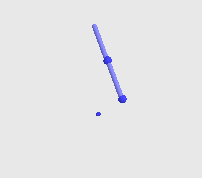
\includegraphics[width=0.3\textwidth]{imagenes/6-neuronal/pend.png}
 \caption{Planar robot in Nengo}
 \label{fig:pend}
\end{figure}
\section{Conclusion}
We built a brain that makes an adaptive control and a PD+G controller. We had some problems with connecting Matlab, then we couldn't make the Nengo simulation complete. Now we are working with the robot computed in Nengo to complete the simulation and adjust the controllers.\\

Without connecting with the robot, the values of the regressor $Y$ and the error $\sigma$ are approximately the same as the Matlab simulation. The output value of the integral depends of the robot manipulator. The PD+G controller worked approximately the same as in Matlab.\\

The brain in Nengo requires a computer with good processor because it consumes a lot of energy. It makes us think the fantastic qualities that a real brain have against a computer.
\bibliographystyle{model1-num-names}
\bibliography{bibliografias/6-neuronal}


% \end{document}
